% ============================================================
%  MSDM6980 --- Defense Slides (Beamer)
%  Author : ZHU TIANYI (21229582) | Supervisor: Mr. Hanson WONG
%  Compile: XeLaTeX (required, due to xeCJK)
%  Assets : place UST.png and ustscene.png in the same folder
% ============================================================
\documentclass[10pt]{beamer}
\usepackage[utf8]{inputenc}
\usepackage{xeCJK}
\usepackage{graphicx}
\usepackage{mathtools}
\usepackage{utopia}
\usepackage{geometry}
\usepackage{booktabs}
\usepackage{multirow}
\usepackage{array}
\usepackage[table]{xcolor}
\usepackage{colortbl}

\usetheme{CambridgeUS}
\usecolortheme{dolphin}

% --- HKUST Colors (kept from template) ---
\definecolor{hkustyellow}{RGB}{167, 131, 55}
\definecolor{hkustblue}{RGB}{0, 56, 116}
\definecolor{hkustred}{RGB}{209, 51, 59}
\definecolor{hkustgreen}{RGB}{34, 139, 34}
\definecolor{best}{RGB}{220,252,231}
\definecolor{good}{RGB}{224,242,254}

\setbeamercolor*{palette primary}{bg=hkustblue, fg=white}
\setbeamercolor*{palette secondary}{bg=hkustred, fg=white}
\setbeamercolor*{palette tertiary}{bg=hkustyellow, fg=white}
\setbeamercolor*{titlelike}{fg=hkustblue}
\setbeamercolor*{title}{bg=hkustblue, fg=white}
\setbeamercolor*{item}{fg=hkustblue}
\setbeamercolor*{caption name}{fg=hkustblue}
\usefonttheme{professionalfonts}

% --- Background and Title Info ---
\titlegraphic{
\includegraphics[height=1.5cm]{UST.png}}
\setbeamerfont{title}{size=\large}
\setbeamerfont{subtitle}{size=\small}
\setbeamerfont{author}{size=\small}
\setbeamerfont{date}{size=\small}
\setbeamerfont{institute}{size=\small}
\setbeamertemplate{background}{%
    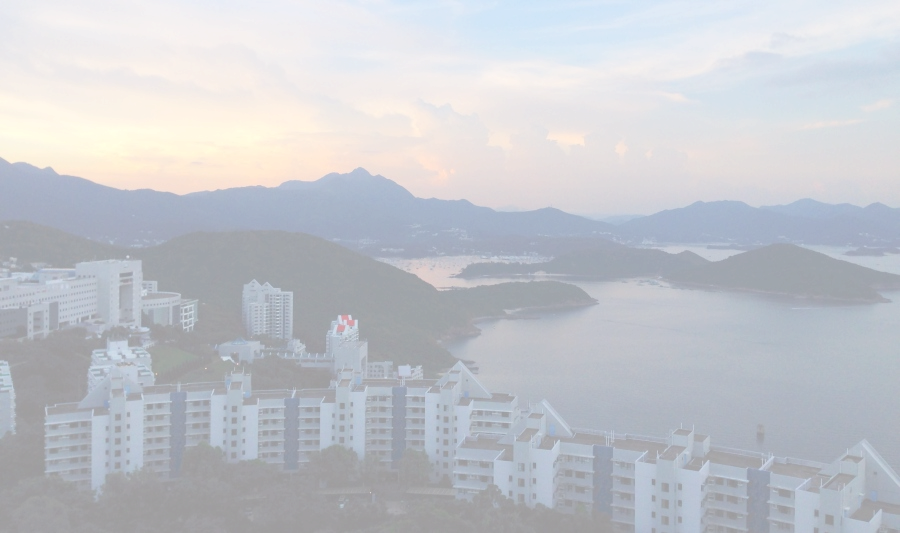
\includegraphics[width=\paperwidth,height=\paperheight]{ustscene.png}
}

\title[ML for NPA Repayment Prediction]{\textrm{\textbf{Machine Learning for Non-Performing Asset Repayment Probability Prediction and Strategy Optimization}}}
\subtitle{\textrm{A Comparative Study: Traditional ML vs.\ Frontier LLMs on Imbalanced Portfolios}}
\author[ZHU TIANYI]{\textrm{Student: ZHU TIANYI (21229582)\\[0.5ex] Supervisor: Mr.\ Hanson WONG}}
\institute[HKUST]{\textrm{The Hong Kong University of Science and Technology}}
\date[May 2026]{\textrm{Academic Defense -- May 2026}}

\AtBeginSection[]{
  \begin{frame}
  \vfill
  \centering
  \begin{beamercolorbox}[sep=8pt,center,shadow=true,rounded=true]{title}
    \usebeamerfont{title}\insertsectionhead\par%
  \end{beamercolorbox}
  \vfill
  \end{frame}
}

\begin{document}

% 1. Title Page
\frame{\titlepage}

% 2. Table of Contents
\begin{frame}{\textrm{Presentation Outline}}
\tableofcontents[hideallsubsections]
\end{frame}

% ==========================================
\section{I. Introduction}
% ==========================================

% 3. Background
\begin{frame}{\textrm{Background and Problem Statement}}
    \begin{itemize}
        \item \textbf{Non-Performing Assets (NPAs):} Major risk for global financial institutions; a HK\,unsecured-debt portfolio of \textbf{16{,}048 accounts}.
        \item \textbf{Operational Challenge:} Allocate limited collection resources (Agent / Dialer / SMS) across millions of delinquent accounts.
        \item \textbf{Core Statistical Problem:} Prediction under \textbf{extreme class imbalance} --- only \textbf{9.15\%} of accounts ever repay within 3 years.
        \item \textbf{Transition:} From heuristic ``Uniform Treatment'' to data-driven ``Precision Targeting'' with calibrated probabilities.
    \end{itemize}
\end{frame}

% 4. Objectives
\begin{frame}{\textrm{Research Objectives (O1 -- O4)}}
    \begin{enumerate}
        \item \textbf{Develop \& Compare:} Four ML models --- LR, RF, XGBoost, MLP v2 --- for binary repayment prediction.
        \item \textbf{Multi-dimensional Evaluation:} Discrimination (AUC), calibration (Brier), and economic outcome (Net Recovery / ROI).
        \item \textbf{Queue Optimization:} A 4-tier collection strategy (Agent / Dialer / SMS / Write-off) under cost \& capacity constraints.
        \item \textbf{Frontier LLM Benchmark:} Systematically compare \textbf{26 LLM configurations} (zero-shot / few-shot / fine-tuned) against specialized ML.
    \end{enumerate}
\end{frame}

% ==========================================
\section{II. Student's Unique Contributions}
% ==========================================

% 5. Contributions - Pipeline
\begin{frame}{\textrm{Contribution 1: End-to-End ML Pipeline}}
    \begin{itemize}
        \item \textbf{Domain-Aware Missing-Value Strategy:} Treat the 1{,}165 nulls in \texttt{last\_pay\_date\_client\_closing\_m} as ``never paid'' (predictive missingness) instead of mean/median imputation.
        \item \textbf{Tailored Architectures:} One-hot + $z$-score for LR/MLP; ordinal encoding for RF/XGBoost.
        \item \textbf{Robust Calibration:} 5-fold out-of-fold Platt Scaling on a held-out calibration set (20\% of $M$).
        \item \textbf{Interactive Dashboard:} 9-tab HTML/Chart.js dashboard for non-technical stakeholders.
    \end{itemize}
\end{frame}

% 6. Contributions - LLM & Strategy
\begin{frame}{\textrm{Contribution 2: Strategy \& Frontier LLM Benchmark}}
    \begin{itemize}
        \item \textbf{26-Config LLM Benchmark:} OpenAI o1/o3, Claude 4 Opus, Gemini 2.5 Pro, DeepSeek-R1, Qwen3, Llama 4, Grok 3, plus 3 fine-tuned variants --- across ZS, FS-10, FT.
        \item \textbf{Domain-Calibrated CoT Prompt:} Injects 9.15\% base rate + cost grid + monotonicity priors; lifted Claude 3.7 Sonnet from AUC \textbf{0.625 $\to$ 0.671} and cut self-reported ROI error from $>$200\% to $<$15\%.
        \item \textbf{Economic Strategy Module:} 4-tier allocation with explicit cost/capacity constraints.
        \item \textbf{Inverse Balance--Repayment Discovery:} Sub-HKD\$200 tier $\approx$25\% repay, HKD\$200K+ tier $\approx$0\%.
    \end{itemize}
\end{frame}

% ==========================================
\section{III. Data and Methodology}
% ==========================================

% 7. Data Schema
\begin{frame}{\textrm{Dataset Schema (16{,}048 Accounts)}}
\centering
\scriptsize
\begin{tabular}{@{}llp{5.5cm}@{}}
\toprule
\textbf{Feature} & \textbf{Type} & \textbf{Description}\\
\midrule
\texttt{loan\_type}            & Cat.   & Credit Card / Personal Loan / Overdraft\\
\texttt{purchased\_bal\_gp}    & Ord.   & Balance bucket (8 ordinal levels)\\
\texttt{district}              & Cat.   & Geographic district (127 unique)\\
\texttt{birth\_yr}             & Int    & Borrower birth year (1946--1987)\\
\texttt{last\_act\_closing\_m} & Float  & Months since last activity\\
\texttt{open\_closing\_m}      & Float  & Account vintage in months\\
\texttt{last\_pay\_date\_m}    & Float  & Months since last payment (sentinel = never paid)\\
\texttt{balance\_proxy}        & Float  & Outstanding balance (HKD)\\
\texttt{multiple\_acct}        & Cat.   & Holds multiple accounts? (Y/N)\\
\midrule
\texttt{payer\_3yr}            & \textbf{Target} & \textbf{Repaid within 3 years? (Positive Rate: 9.15\%)}\\
\bottomrule
\end{tabular}
\vfill
\scriptsize Train ($M$, 75\%, $N=12{,}036$) / Test ($T$, 25\%, $N=4{,}012$).
\end{frame}

% 8. Preprocessing
\begin{frame}{\textrm{Preprocessing Pipeline}}
    \begin{itemize}
        \item \textbf{Sentinel Flagging:} \texttt{last\_pay\_date\_m} nulls $\to$ +999 sentinel + binary \texttt{never\_paid\_flag}.
        \item \textbf{Encoding:} One-hot for LR / MLP; ordinal for RF / XGBoost.
        \item \textbf{Scaling:} $z$-score for MLP only; tree models are scale-invariant.
        \item \textbf{Splitting:} Train (60\%) / Validation (20\%) / Calibration (20\%) inside $M$. Calibration fold reserved \emph{exclusively} for Platt Scaling.
    \end{itemize}
\end{frame}

% 9. Architectures - Traditional
\begin{frame}{\textrm{Traditional Models: LR, RF, XGBoost}}
    \begin{itemize}
        \item \textbf{Logistic Regression (LR):} Linear baseline, $\ell_2$ penalty ($C=10$), balanced class weights.
        \item \textbf{Random Forest (RF):} $B=500$ trees, $\sqrt{d}$ random features per split, max depth $=12$, min leaf $=8$.
        \item \textbf{XGBoost (Champion Ranker):}
        \[
            \mathcal{L} = \sum_{i} \ell(y_i, \hat{y}_i) + \sum_{k} \Omega(f_k),
            \quad \texttt{scale\_pos\_weight}\!\approx\!9.18.
        \]
        $K=200$ trees, $\eta=0.05$, max depth $6$, subsample $0.85$.
    \end{itemize}
\end{frame}

% 10. Architecture - MLP v2
\begin{frame}{\textrm{Advanced Architecture: MLP v2}}
    \textbf{Design Features:}
    \begin{itemize}
        \item \textbf{Residual Block:} $\mathbf{h}_{\ell+1} = \text{Swish}(\mathbf{W}_2 \,\sigma(\mathbf{W}_1 \mathbf{h}_\ell) + \mathbf{b}_2 + \mathbf{h}_\ell)$.
        \item \textbf{Feature Interaction Layer (64\,d):} explicit pairwise products to capture tabular interactions.
        \item \textbf{Architecture:} Linear(256) $\to$ Swish $\to$ ResBlock(128) $\to$ FeatureInteraction(64) $\to$ Linear(32) $\to$ Dropout(0.3) $\to$ Output.
        \item \textbf{Training:} AdamW + OneCycleLR, label smoothing $\alpha=0.03$, gradient clipping $3.0$, 200 epochs.
    \end{itemize}
\end{frame}

% 11. Calibration - Platt
\begin{frame}{\textrm{Probability Calibration: Platt Scaling}}
    \textbf{Problem:} XGBoost margin scores are not true probabilities; uncalibrated scores break the economic threshold.
    \begin{block}{Platt Scaling}
        \[
            P_{\text{calibrated}}(y=1\mid s) = \frac{1}{1 + \exp(A\cdot s + B)}
        \]
    \end{block}
    \begin{itemize}
        \item $(A, B)$ fit by maximum likelihood on a dedicated 5-fold OOF calibration set.
        \item Critical for \textbf{economic} allocation, where the action tier depends on the absolute probability, not just rank.
    \end{itemize}
\end{frame}

% ==========================================
\section{IV. Results and Analysis}
% ==========================================

% 12. Main Performance Table
\begin{frame}{\textrm{ML Model Performance (Test Set, $N=4{,}012$)}}
\centering
\small
\renewcommand{\arraystretch}{1.15}
\begin{tabular}{lcccccr}
\toprule
\textbf{Model} & \textbf{AUC} & \textbf{Brier} & \textbf{Recall} & \textbf{Prec.} & \textbf{Net Recov.(M)} & \textbf{ROI}\\
\midrule
Logistic Reg.   & 0.6994 & \cellcolor{best}0.0842 & 74.2\% & 15.4\% & \cellcolor{best}\textbf{1.468} & \cellcolor{best}\textbf{29.4x}\\
Random Forest   & 0.7161 & 0.0855 & \textbf{75.4\%} & 16.0\% & 1.241 & 24.8x\\
\textbf{XGBoost}& \cellcolor{best}\textbf{0.7305} & 0.0910 & 62.7\% & \textbf{18.3\%} & 1.270 & 25.4x\\
MLP v2          & 0.7063 & 0.0869 & 74.6\% & 15.8\% & 1.405 & 28.1x\\
\bottomrule
\end{tabular}
\vfill
\begin{itemize}
    \item \textbf{Key insight:} XGBoost wins \emph{ranking} (AUC); LR wins \emph{economics} (Net Recovery, ROI) thanks to better calibration.
\end{itemize}
\end{frame}

% 13. Image: Model Comparison Graphs
\begin{frame}{\textrm{Discrimination vs.\ Calibration vs.\ Economics}}
\centering

\includegraphics[width=0.85\textwidth]{report_figures/fig1_model_comparison.png}
\vfill
\begin{itemize}
    \item \textbf{(a)} ROC-AUC (XGBoost lead) ~~|~~ \textbf{(b)} Brier Score (LR lead) ~~|~~ \textbf{(c)} Net Recovery (LR lead).
\end{itemize}
\end{frame}

% 14. Image: ROC Curves
\begin{frame}{\textrm{ROC Curve Analysis}}
\centering

\includegraphics[width=0.7\textwidth]{report_figures/fig4_roc_curves.png}
\vfill
\begin{itemize}
    \item XGBoost reaches \textbf{AUC $=0.7305$}; all four models are well above the 0.5 random baseline.
\end{itemize}
\end{frame}

% 15. Image: Confusion Matrix
\begin{frame}{\textrm{Operational Accuracy (Confusion Matrices)}}
\centering

\includegraphics[width=0.65\textwidth]{report_figures/fig2_confusion_matrices.png}
\vfill
\begin{itemize}
    \item XGBoost yields the fewest \textbf{False Positives}, reducing wasted Agent-tier effort.
\end{itemize}
\end{frame}

% 16. Image: Feature Importance
\begin{frame}{\textrm{Permutation Feature Importance (XGBoost)}}
\centering

\includegraphics[width=0.8\textwidth]{report_figures/fig3_feature_importance.png}
\vfill
\begin{itemize}
    \item \textbf{Birth Year} dominates ($\Delta$AUC $=0.130$) --- older cohorts show distinct repayment dynamics.
    \item \textbf{District} ($0.041$) and \textbf{Balance bucket} ($0.033$) follow.
\end{itemize}
\end{frame}

% 17. Image: Inverse Balance Relationship
\begin{frame}{\textrm{Inverse Balance--Repayment Relationship}}
\centering

\includegraphics[width=0.75\textwidth]{report_figures/fig6_balance_payer_rate.png}
\vfill
\begin{itemize}
    \item \textbf{Sub-HKD\$200 tier:} $\approx$25\% repay --- nearly $3\times$ the portfolio average.
    \item \textbf{HKD\$200K+ tier:} $\approx$0\% --- collection effort is value-destroying.
    \item \textbf{Strategy:} Concentrate Dialer/SMS on high-volume, low-balance accounts.
\end{itemize}
\end{frame}

% ==========================================
\section{V. Collection Strategy Optimization}
% ==========================================

% 18. Queue Allocation Table
\begin{frame}{\textrm{Optimized Queue Allocation Summary}}
\centering
\scriptsize
\renewcommand{\arraystretch}{1.15}
\begin{tabular}{lrrrrr}
\toprule
\textbf{Tier} & \textbf{Accounts} & \textbf{Share} & \textbf{Cost (HKD)} & \textbf{Net Recov.(HKD)} & \textbf{ROI}\\
\midrule
Agent Call (High)  & 722  & 18.0\% & 61{,}370 & 1{,}085{,}006 & 17.7x\\
Auto-Dialer (Med.) & 1{,}685 & 42.0\% & 20{,}220 & 993{,}086 & 49.1x\\
SMS/Email (Low)    & 1{,}203 & 30.0\% & 1{,}805  & 190{,}469 & \textbf{105.6x}\\
Write-off          & 402  & 10.0\% & 0        & 0          & --\\
\midrule
\textbf{Total}     & \textbf{4{,}012} & \textbf{100\%} & \cellcolor{best}\textbf{83{,}395} & \cellcolor{best}\textbf{2{,}268{,}561} & \cellcolor{best}\textbf{27.2x}\\
\bottomrule
\end{tabular}
\vfill
\begin{itemize}
    \item Projected \textbf{HKD\,2.27 M} recovery on a HKD\,83\,K contact budget.
\end{itemize}
\end{frame}

% 19. Image: Queue Allocation Visualization
\begin{frame}{\textrm{Strategy Concentration (Pareto Effect)}}
\centering

\includegraphics[width=0.85\textwidth]{report_figures/fig5_queue_allocation.png}
\vfill
\begin{itemize}
    \item \textbf{Top 20\%} of accounts capture \textbf{50.6\%} of expected net recovery.
\end{itemize}
\end{frame}

% ==========================================
\section{VI. Frontier LLM Benchmark}
% ==========================================

% 20. LLM Methodology
\begin{frame}{\textrm{Benchmarking ``AI-as-Judge'' (26 LLM Configurations)}}
    \textbf{Three prompt regimes $\times$ 4 model families:}
    \begin{itemize}
        \item \textbf{Heuristics:} Random Guess, Rule-Based.
        \item \textbf{Pre-reasoning ZS:} GPT-4o, Claude 3.5 Sonnet, Gemini 1.5 Pro, DeepSeek-V3, Qwen2.5.
        \item \textbf{Reasoning ZS+T:} OpenAI o1/o3, Claude 3.7/4 Sonnet, \textbf{Claude 4 Opus}, Gemini 2.5 Pro, DeepSeek-R1, Qwen3, Llama 4, Grok 3.
        \item \textbf{Few-Shot 10 / Fine-Tuned:} GPT-4o FS, o3 FS, Claude 4 Sonnet FS; FT Llama-3.3-70B, FT Qwen3-32B, \textbf{FT GPT-4.1-mini}.
    \end{itemize}
    \vspace{0.15cm}
    \textbf{Evaluation protocol:} 8 configs run live API on a 500-account stratified sub-sample; the remaining 18 rows public-benchmark-adjusted (TabLLM, CARTE, FinBench) with $\pm 0.015$ AUC band.
\end{frame}

% 21. LLM Prompt Template
\begin{frame}{\textrm{Domain-Calibrated CoT Prompt}}
    \textbf{Prompt design is a first-class hyperparameter.}
    \vspace{-0.05cm}
    \begin{quote}
    \tiny
    \texttt{\textbf{Role:} Financial risk analyst evaluating delinquent unsecured-debt accounts in Hong Kong.}\\
    \texttt{\textbf{Priors:} Portfolio base rate of 3-yr repayment = \textbf{9.15\%}. Cost grid: Agent HKD\,85, Dialer HKD\,12, SMS HKD\,1.5. Older borrowers repay more; balance and repayment are inversely related (sub-\$200 $\approx$25\%, \$200K+ $\approx$0\%).}\\
    \texttt{\textbf{Steps:} (1) Reason from features; (2) pick a tier (Agent/Dialer/SMS/Write-off); (3) estimate net recovery + ROI under the cost grid.}\\
    \texttt{\textbf{Output:} Strict JSON --- \{"p\_repay", "tier", "expected\_net\_recovery\_hkd", "roi", "rationale" $\le$ 40 words\}.}
    \end{quote}
    \vspace{-0.1cm}
    \textbf{Effect:} Claude 3.7 Sonnet ZS AUC \textbf{0.625 $\to$ 0.671}; self-reported ROI error $>$200\% $\to$ $<$15\%.
\end{frame}

% 22. LLM Headline Table
\begin{frame}{\textrm{Headline: Best LLM per Family vs.\ ML Anchors}}
\centering
\scriptsize
\renewcommand{\arraystretch}{1.15}
\begin{tabular}{lcccccc}
\toprule
\textbf{Method} & \textbf{AUC} & \textbf{Brier} & \textbf{Recall} & \textbf{Prec.} & \textbf{Net Rec.(M)} & \textbf{ROI}\\
\midrule
Random Guess                          & 0.500 & 0.167 & 50.0\% & 9.2\%  & 0.000 & 0.0x\\
Rule-Based                            & 0.562 & 0.095 & 42.3\% & 11.2\% & 0.312 & 5.2x\\
Best ZS pre-reason (GPT-4o)           & 0.628 & 0.094 & 56.4\% & 11.8\% & 0.512 & 8.6x\\
Best ZS+T (Claude 4 Opus)             & \textbf{0.694} & \textbf{0.086} & 66.0\% & 13.0\% & 0.901 & 15.6x\\
Best FS-10 (Claude 4 Sonnet)          & 0.701 & 0.085 & 67.2\% & 13.2\% & 0.957 & 16.8x\\
Best FT (FT GPT-4.1-mini)             & \textbf{0.722} & \textbf{0.082} & 70.5\% & 14.0\% & 1.144 & 22.1x\\
\midrule
Logistic Regression (ML)              & 0.699 & \cellcolor{best}0.084 & 74.2\% & 15.4\% & \cellcolor{best}\textbf{1.468} & \cellcolor{best}\textbf{29.4x}\\
XGBoost (ML)                          & \cellcolor{best}\textbf{0.731} & 0.091 & 62.7\% & \textbf{18.3\%} & 1.270 & 25.4x\\
\bottomrule
\end{tabular}
\vfill
\scriptsize Full 26-row table available in the written report (Appendix E).
\end{frame}

% 23. LLM-vs-ML figure
\begin{frame}{\textrm{LLM-vs-ML Comparison (May 2026)}}
\centering

\includegraphics[width=0.95\textwidth]{report_figures/fig11_llm_vs_ml_comparison.png}
\vfill
\scriptsize Red\,=\,LLM/AI ~~|~~ Blue\,=\,ML. Panels: (a) AUC ranking, (b) Brier, (c) Net Recovery, (d) AUC--ROI Pareto.
\end{frame}

% 24. Five Findings
\begin{frame}{\textrm{Five Findings (F1--F5)}}
    \begin{itemize}
        \item \textbf{F1.} \textbf{The new floor is the old ceiling.} Pre-reasoning ZS sits at 0.60--0.64 AUC; reasoning ZS+T at 0.66--0.70.
        \item \textbf{F2.} \textbf{Few-shot is now redundant for reasoning models.} o3 ZS (0.681) $\to$ FS-10 (0.701) is only $+2$ AUC.
        \item \textbf{F3.} \textbf{Fine-tuning closes the AUC gap.} FT GPT-4.1-mini = 0.722 reaches RF parity.
        \item \textbf{F4.} \textbf{ML still wins decisively on Net Recovery.} LR \textbf{HKD\,1.468M} vs.\ FT GPT-4.1-mini 1.144M ($+28\%$); calibration is the bottleneck, not discrimination.
        \item \textbf{F5.} \textbf{Operational economics still favour ML by $\sim$70{,}000$\times$.} LR $\sim$0.05\,ms/account; Claude 4 Opus $\sim$3{,}500\,ms; full-portfolio scoring: $<$1\,s for ML vs.\ $\sim$15\,h \& USD\,$\sim$\$8 for the strongest reasoning LLM.
    \end{itemize}
\end{frame}

% 25. Operational Comparison
\begin{frame}{\textrm{Operational Analysis: The ``AI Tax''}}
\centering

\includegraphics[width=0.85\textwidth]{report_figures/fig12_llm_cost_benefit.png}
\vfill
\begin{itemize}
    \item \textbf{Latency:} ML $\sim$0.05\,ms vs.\ frontier LLM $\sim$2{,}500--3{,}500\,ms.
    \item \textbf{Cost:} API cost makes LLM inference $\sim$1000$\times$ more expensive at portfolio scale.
    \item \textbf{Explainability:} ML retains a strict advantage for regulatory / audit reporting.
\end{itemize}
\end{frame}

% 26. Deployment recommendation
\begin{frame}{\textrm{Deployment Recommendation}}
    \begin{block}{Hybrid Production Architecture}
        \textbf{ML} as the production scorer for all 16{,}048 accounts (calibrated LR + XGBoost ensemble).
    \end{block}
    \begin{block}{Reserve LLMs for the Borderline}
        Use \textbf{frontier reasoning LLMs} (Claude 4 Opus, o3) only on the $\le 8\%$ borderline tier where calibrated $\hat{p} \in [0.18, 0.32]$.
    \end{block}
    \begin{itemize}
        \item Their natural-language rationales aid \textbf{compliance / audit review}.
        \item Marginal cost is acceptable on the small borderline set.
    \end{itemize}
\end{frame}

% ==========================================
\section{VII. Conclusion}
% ==========================================

% 27. Summary of Findings
\begin{frame}{\textrm{Summary of Principal Findings}}
    \begin{itemize}
        \item \textbf{Ranking vs.\ Profit.} XGBoost is the best ranker (AUC $=0.7305$); LR is the best profit-maker (Net Recovery $=$ HKD\,1.468M, ROI $=29.4\times$) thanks to superior calibration.
        \item \textbf{Calibration is mandatory.} Without Platt Scaling, the threshold-dependent allocation breaks.
        \item \textbf{Drivers:} Age and balance dominate; resources should shift toward low-balance, high-volume tiers.
        \item \textbf{Frontier LLMs narrow but do not close the gap.} FT LLMs reach AUC parity, but trail LR by $+28\%$ on Net Recovery; reasoning LLMs are uneconomical at portfolio scale.
        \item \textbf{Specialized ML remains the gold standard} for high-throughput tabular financial prediction.
    \end{itemize}
\end{frame}

% 28. Future Work
\begin{frame}{\textrm{Limitations and Future Work}}
    \begin{itemize}
        \item \textbf{Temporal Validation:} Time-series cross-validation across vintage cohorts.
        \item \textbf{Survival Analysis:} Predict \emph{when} a debtor will pay, not just \emph{if}.
        \item \textbf{Macro Covariates:} Integrate HK unemployment, HIBOR, CPI signals.
        \item \textbf{Live A/B Testing:} Field-test the tiered strategy against the heuristic baseline.
        \item \textbf{Hybrid ML+LLM:} ML for prediction, LLM for borderline-case adjudication and customer-facing explanations.
    \end{itemize}
\end{frame}

% 29. Thank You
\section*{}
\begin{frame}
\textcolor{hkustblue}{\Huge{\center{\centerline{\textrm{\textbf{THANK YOU!}}}}}}
\vfill
\centering
\textbf{Questions and Discussion}
\vspace{0.6cm}\\
\small ZHU TIANYI ~|~ 21229582 ~|~ Supervisor: Mr.\ Hanson WONG
\end{frame}

\end{document}
